\chapter{Experiments}
\label{ch:experiments}
This chapter will describe what experiments have been performed to answer the research question formulated in Chapter \ref{ch:introduction}, and give the results of those experiments.
%
The description of the experiments includes implementation details of the methods described in the previous chapter, as well as the strategy employed for the hyper-parameter search.
%
The results are include both performance metrics resulting from the hyper-parameter searches, and  analyses of the methods aimed at confirming the methods are working as intended.

\section{Implementations}
We make the implementations of the methods described in Chapter \ref{ch:methodology} and the experiments described here freely available in the newly created SemKGE (Semantic KGE) repository,\sidenote[][0em]{\rurl{github.com/sfschouten/semantic-kge}} which was developed as a plugin to the LibKGE library\sidenote[][0em]{\rurl{github.com/uma-pi1/kge}}  \mycitep[0em]{broscheit_libkge_2020}.

\subsection{Type-linkprior}
% \todo[inline,caption={}]{
%     \begin{itemize}
%         \item explain learnable lambdas
%         \item 
%     \end{itemize}
% }
This method is implemented such that the variables $\lambda_{head}, \lambda_{relation}, \lambda_{tail}$ from Formulas \ref{formula:p_hrt}, \ref{formula:p_rht}, \ref{formula:p_thr} are learnable during training. As such, we introduce a hyper-parameter to control whether they are learned or not. If this hyper-parameter is set to true, the hyper-parameters that are normally used to set these values, now merely set their initial value.

%\subsection{Type-mean}
%

\subsection{Type-attentive}
The optimal learning rate for training a method like TransE can be quite high (\citeauthor{ruffinelli_you_2019} find an optimal learning rate of 0.25327).
Since the attention mechanism in the type-attentive embedder is the only part of the model that contains fully connected layers (which generally require lower learning rates), we tune the learning rate separately for that component. 


\subsection{Type-embedprior}\label{sec:experiments:impl_type_embedprior}
This method's additional optimization objective maximizes the difference in probability density assigned to an entity-embedding by that entity's types' distributions, and the density assigned by the other types' distributions.
We implement this by drawing one negative type sample for each type of each entity.


\subsection{Additional losses with constrained optimization.}
Optimizing with multiple objectives is often done by creating a weighted sum of loss terms.
But this strategy may be flawed, recently it was shown that this approach may fail even on small toy problems \mycitep{degrave_how_2021}. %mayne \sidenote on pareto front.
A potential solution is to construct a constrained optimization problem, where we identify one of our loss terms as the primary objective and incorporate the others as constraints. 
Using the Modified Differential Method of Multipliers \mycitep{platt_constrained_1987} allows us to utilize gradient descent with such a constrained optimization problem.
This method has been employed successfully with Variational Autoencoders \mycitep{rezende_taming_2018}, but should lead to more easily tunable hyperparameters regardless of the application.

As such the type-attentive's mutual information loss, and the type-embedprior's type-distribution density loss are both incorporated as constraints.


% \begin{align}
%     \argmax_{\epsilon, \mu, \sigma} \quad 
% &   p( x | \vec{h}, \vec{r}, \vec{t} ) \\[0.4em]
%     \text{subject to} \quad 
% &   u < \prod_{C_{h,s}} f_{\vec{C}_{s}} ( \vec{h} ) 
%       - \prod_{\lnot C_{h,s}} f_{\vec{C}_{s}} ( \vec{h} )\\
%     \text{and} \quad
% &   v < \prod_{C_{t,s}} f_{\vec{C}_{s}} ( \vec{t} )
%       - \prod_{\lnot C_{t,s}} f_{\vec{C}_{s}} ( \vec{t} ).
% \end{align}


\section{Datasets}
The datasets we use for our experiments are FB15K-237 \mycitep{toutanova_representing_2015}, WN18RR \mycitep{dettmers_convolutional_2018}, CoDEx-S and CoDEx-M \mycitep{safavi_codex_2020}.
%
The first two are well known benchmarks for Link Prediction \mycitep{ruffinelli_you_2019}.
They are the successors of the FB15K and WN18 datasets, which had been found to have test leakage \mycitep{rossi_knowledge_2021}.
The latter are two variants of a recently introduced set of benchmarks called CoDEx.  \citeauthor{safavi_codex_2020} show that CoDEx covers more diverse and interpretable content than FB15K-237, and that CoDEx is a more difficult . 
Statistics for each of these datasets can be seen in Table \ref{tab:dataset_statistics}.

%   \multirow{2}{*}{\fbox{\parbox[t][2.3em][s]{4.40em}{types\\per entity}}} &
%   \multirow{2}{*}{\fbox{\parbox[t][2.3em][s]{2.75em}{types\\in use}}} &
%   \multirow{2}{*}{\fbox{\parbox[t][2.3em][s]{2.50em}{total\\types}}} \\
\vspace{3cm}
\begin{table*}
\centering
    \begin{tabular}{@{}lrrrrrrrr@{}}
    \toprule
    \multirow{2}{*}{} &
      \multicolumn{1}{l}{\multirow{2}{*}{entities}} &
      \multicolumn{1}{l}{\multirow{2}{*}{relations}} &
      \multicolumn{3}{l}{triples} &
      \multirow{2}{*}{\parbox{4.70em}{\vspace{4pt}\setstretch{0.8}avg. types\\per entity}} &
      \multirow{2}{*}{\parbox{2.75em}{\vspace{1pt}\setstretch{0.8}types\\in use}} &
      \multirow{2}{*}{\parbox{2.50em}{\vspace{3pt}\setstretch{0.8}total\\types}} \\
    \cmidrule(lr){4-6}
     &
      \multicolumn{1}{l}{} &
      \multicolumn{1}{l}{} &
      \multicolumn{1}{l}{train} &
      \multicolumn{1}{l}{valid} &
      \multicolumn{1}{l}{test} &
       &
       \\ \midrule
    FB15K-237 & 14,541 & 237 & 272,115 & 17,535 & 20,466 & 12.422 & 3,865 & 4,054 \\
    WN18RR    & 40,943 &  11 &  86,835 &  3,034 &  3,134 &  1.000 &     4 &     4 \\
    CoDEx-S   &  2,034 &  42 &  32,888 &  1,827 &  1,828 &  1.619 &   502 & 3,443 \\
    CoDEx-M   & 17,050 &  51 & 185,584 & 10,310 & 10,311 &  1.253 & 1,505 & 3,443 \\ 
    \bottomrule
    \end{tabular}\vspace{1em}
\caption{Dataset statistics.}
\label{tab:dataset_statistics}
\end{table*}



\begin{figure*}
    \centering
    \begin{subfigure}[b]{0.32\textwidth}
        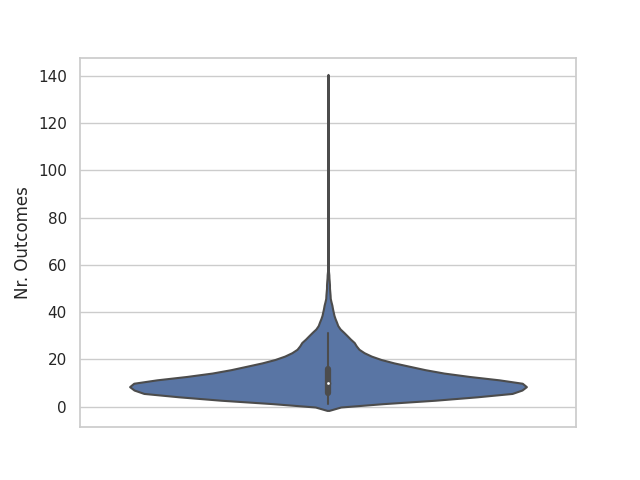
\includegraphics[trim=0cm 11mm 1cm 0pt, clip]{figures/datasets/fb15k-237.png}
        \caption{FB15K-237}
    \end{subfigure}
    \begin{subfigure}[b]{0.32\textwidth}
        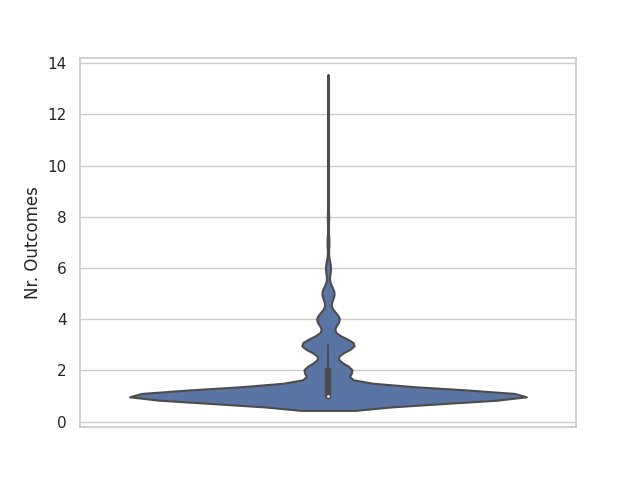
\includegraphics[trim=0cm 11mm 1cm 0pt, clip]{figures/datasets/codex-s.png}
        \caption{CoDEx-S}
    \end{subfigure}
    \begin{subfigure}[b]{0.32\textwidth}
        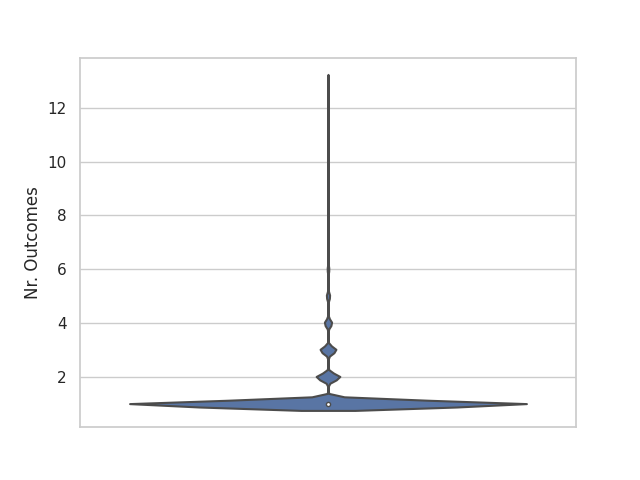
\includegraphics[trim=0cm 11mm 1cm 0pt, clip]{figures/datasets/codex-m.png}
        \caption{CoDEx-M}
    \end{subfigure}
    \caption[Distribution of number of types per entity.]{Distribution of number of types per entity across test portion of the datasets. The WN18RR dataset is omitted because it has exactly one type for each entity.}
    \label{fig:my_label}
\end{figure*}

%\FloatBarrier


\section{Technical Details}
All experiments were run on the SURFsara Lisa GPU cluster\sidenote[][2cm]{\rurl{userinfo.surfsara.nl/systems/lisa/description}}. 
The nodes we used had Nvidia GeForce 1080Ti GPUs with 11GB of VRAM.


\section{Evaluating \& Optimizing Link Prediction}
The Link Prediction task is evaluated as a ranking problem. Given a triple we know to be correct $(h, r, t)$ (those triples in the validation or test set), we use our model to predict what the head or tail should be, i.e. $(?, r, t)$ and $(h, r, ?)$. We rank all other entities on their likelihood of being the missing head or tail. 
The ranking that the model predicts is evaluated by what ranks are assigned to the original correct head and tail.

\paragraph{Evaluation metrics} used to quantify the quality of the rankings include: Mean Rank (MR), Mean Reciprocal Rank (MRR), and Hits@N.
The Mean Rank is the mean of the ranks assigned to the correct triples. This metric gives a number between one and the number of entities, the lower the better.
It is easily interpreted, but its sensitivity to outliers is causing it to be abandoned in favor of MRR \mycitep[]{rossi_knowledge_2021}.
The Mean Reciprocal Rank is the mean of multiplicative inverse of the ranks. It gives a number between 0 and 1, the higher the better. It is much less sensitive to outliers.
Hits@N gives the percentage of correct triples with an assigned rank below N, the higher the better.

These metrics can be calculated in two different ways, they can be computed \textit{raw} or \textit{filtered}. This choice determines how we treat other predictions of heads/tails that also correct triples, that are not the triple for which we are currently doing head/tail prediction. If we report the \textit{raw} metrics, we leave these other correct triples alone, if we report the \textit{filtered} metrics we filter them out. The \textit{filtered} metrics are generally preferred because we do not care about the model ranking other correct triples above the currently evaluated triple.

\paragraph{Loss functions} used to optimize for these ranking metrics need special attention, because the metrics themselves are not continuous. This is because these metrics require sorting the scores assigned to triples in order to compute their rank. So to optimize with gradient descent, we use separate loss functions as a proxy for these metrics. 

One possibility is to model the truth of a triple as being sampled from a Bernoulli distribution.  
\begin{align}
    & X | \vec{h}, \vec{r}, \vec{t}
&& \sim \text{Bernoulli}( \sigma( score( \vec{h}, \vec{r}, \vec{t} ) ) )
\end{align}
Where $\sigma$ is a function that maps the scores to $(0,1)$.
The difference between the model distribution and the data distribution is then quantified as the Binary Cross Entropy (BCE) loss.

Alternatively we can think of the true triples as being sampled from a set of triples $\mathcal{S}_{(h,r,t)}$.
\begin{align}
    & p(\bm{\mathcal{S}}_{(h,r,t)})  && = \sigma \left(  score(\vec{h'}, \vec{r'}, \vec{t'}) \,|\, (\vec{h'}, \vec{r'}, \vec{t'}) \in \bm{\mathcal{S}}_{(h,r,t)} \right)^\top
\\
    & K^+ | \bm{\mathcal{S}}_{(h,r,t)} && \sim \text{Categorical}(|\bm{\mathcal{S}}_{(h,r,t)}|, p(\bm{\mathcal{S}}_{(h,r,t)}))
\\
    & X^{(k')} && = [k' = k^+]
\end{align}
Where $\sigma$ is the softmax function, $S_{(h,r,t)}$ is the set of triples and $\vec{S}_{(h,r,t)}$ are their embeddings. In practice this set is based on a triple $(h,r,t) \in \mathcal{D}^+$, it includes that triple itself and a set of negative triples constructed from the original.
When modeled this way the difference between the model and data distribution is quantified as the Categorical Cross Entropy loss.

Other loss functions like Margin Ranking and Squared error are sometimes also used. However, in contrast to the losses mentioned above, these others are optimal for none of the methods included in the hyper-parameter search performed by \citeauthor{ruffinelli_you_2019}.

\paragraph{Training approaches} differ from each other by how batches of triples are constructed. Negative sampling is an approach that first samples triples from the training data, and then constructs set of negatives for each triple by corrupting one of the triple's components. \citeauthor{ruffinelli_you_2019} implement two other approaches, 1vsAll, and KvsAll. The 1vsAll approach is similar to negative sampling but adds every possible way of corrupting a triple as a negative, even if the resulting triples occur in the training data. 
The KvsAll approach only corrupts either the head or tail, and contrary to 1vsAll, labels all that occur in the training data as positive, and only those that do not as negative.

\section{Hyper-parameter Searches}
Our main experiment is an extensive hyper-parameter search. 
For each of the methods described in Chapter \ref{ch:methodology}, we use TransE as the underlying KGE model.
%
The strategy employed for the hyper-parameter searches is based on the strategy used in \mycite[4em]{ruffinelli_you_2019}. Each search is based on 30 rounds of parameters drawn from a Sobol sequence \mycitep[]{sobol1967distribution}. \citeauthor{ruffinelli_you_2019} follow this with 15 rounds of Bayesian optimization, but since they report that this has minimal effect we do not include these rounds. %\todo{decide definitively}


\subsection{Training}
We use a Categorical Cross Entropy loss, minimizing the KL Divergence between the model and data distributions, and use negative sampling as our training strategy. These two decisions were shown by \citeauthor{ruffinelli_you_2019} to be optimal for the TransE KGE model. 

We use a `shared' implementation of negative-sampling, meaning that the same negative samples are used for each triple in a batch. Note that it is ensured that a triple does not get itself as a negative.

\paragraph{}\noindent%
An extensive overview of which hyper-parameters were tuned can be found in Appendix \ref{apx:hyperparameter_search}

\begin{table}[p]
    \def\fn{\hspace{2pt}} % footnote columns
    \setlength{\tabcolsep}{5pt}
    \centering
    \begin{tabular}{lr@{\fn}lr@{\fn}lr@{\fn}lr@{\fn}l}
        \toprule
        \textit{name}
        &\multicolumn{2}{l}{WN18RR}
                    &\multicolumn{2}{l}{FB15K-237}   
                           & \multicolumn{2}{l}{CoDEx-S}   
                                        & \multicolumn{2}{l}{CoDEx-M} \\
        \cmidrule{1-9}
        non-semantic        & 0.226 && 0.308    && 0.354    && 0.306   \\
        \cmidrule{1-9}
        type-linkprior-only & 0.000 && 0.140    && 0.094    && 0.051   \\
        type-linkprior      & 0.191 && 0.324    && 0.354    && 0.284   \\
        \cmidrule{1-9}
        type-mean           & 0.723 && 0.272    && 0.446    && 0.357   \\
        type-mean+          & 0.174 && 0.319    && 0.350    && 0.274   \\
        type-attentive      & -     &&\textbf{0.615}&%\footnotemark
                                                 &\textbf{0.612}
                                                            &&\textbf{0.477}   \\
        type-attentive-alt  &\textbf{0.816}
                                    && 0.298    && 0.341    && 0.456   \\
        \cmidrule{1-9}
        type-embedprior     & 0.243 && 0.316    && 0.378    && 0.298   \\
        \bottomrule
    \end{tabular} \vspace{1em}
    \caption[MRR obtained by each method for best set of hyperparameters.]{Mean Reciprocal Rank obtained by each method for best set of hyperparameters. } \label{tab:hyperparam-search-results1}
\end{table}
%\addtocounter{footnote}{-1}
%\marginnote{\textsuperscript{\thefootnote\ }test}
%\todo{} 
%\addtocounter{footnote}{1}
%\marginnote{\textsuperscript{\thefootnote\ }test}


\begin{table}[p]
    \def\fn{\hspace{2pt}} % footnote columns
    \setlength{\tabcolsep}{5pt}
    \centering
    \begin{tabular}{lr@{\fn}lr@{\fn}lr@{\fn}lr@{\fn}l}
        \toprule
        \textit{name}
                &\multicolumn{2}{c}{WN18RR}
                            &\multicolumn{2}{c}{FB15K-237}   
                                           & \multicolumn{2}{c}{CoDEx-S}   
                                                                & \multicolumn{2}{c}{CoDEx-M} \\
        \cmidrule{1-9}
        non-semantic         & 1774.06     && 176.93       && \textbf{43.78}            && \textbf{289.89}   \\
        \cmidrule{1-9}
        type-linkprior-only  & 19581.08    && 686.44	   && 290.47           && 4655.25  \\
        type-linkprior       & 4617.39   && \textbf{158.69}       && 49.45     && 434.35   \\
        \cmidrule{1-9}
        type-mean            & 9714.45     && 233.67       && 88.20            && 1959.57  \\
        type-mean+           & 5912.00     && 171.31       && 54.84            && 582.91   \\
        type-attentive       & -           && 5374.72        &%\footnotemark
                                                           & 78.17             && 984.77   \\
        type-attentive-alt   & \textbf{1557.96}     && 188.45       && 54.46            && 967.30   \\
        \cmidrule{1-9}
        type-embedprior      & 3185.04     && 171.81       && 46.87            && 571.06   \\
        \bottomrule
    \end{tabular} \vspace{1em}
    \caption[MR obtained by each method for best set of hyperparameters.]{Mean Rank obtained by each method for set of hyperparameters with highest MRR.} \label{tab:hyperparam-search-results2}
\end{table}
%\addtocounter{footnote}{-1}
%\marginnote{\textsuperscript{\thefootnote\ }test}
%\addtocounter{footnote}{1}
%\marginnote{\textsuperscript{\thefootnote\ }test}

\begin{table}[p]
    \def\fn{\hspace{2pt}} % footnote columns
    \setlength{\tabcolsep}{5pt}
    \centering
    \begin{tabular}{lr@{\fn}lr@{\fn}lr@{\fn}lr@{\fn}l}
        \toprule
        \textit{name}
                &\multicolumn{2}{c}{WN18RR}
                            &\multicolumn{2}{c}{FB15K-237}   
                                           & \multicolumn{2}{c}{CoDEx-S}   
                                                                & \multicolumn{2}{c}{CoDEx-M} \\
        \cmidrule{1-9}
        non-semantic         & 51.53    && 49.90    && 64.37    && 46.65  \\
        \cmidrule{1-9}
        type-linkprior-only  & 00.00    && 21.91	&& 18.56    && 7.85   \\
        type-linkprior       & 43.75	&& 51.14    && 58.73    && 44.68    \\
        \cmidrule{1-9}
        type-mean            & 72.33    && 40.89    && 64.50    && 47.21  \\
        type-mean+           & 42.55    && 49.02    && 57.85    && 42.22  \\
        type-attentive       & -        && \textbf{61.57}     &%\footnotemark
                                                    & \textbf{83.03}     && \textbf{54.09}  \\
        type-attentive-alt   & \textbf{82.23}    && 47.05    && 58.35    && 51.85  \\
        \cmidrule{1-9}
        type-embedprior      & 63.25    && 49.57    && 62.62    && 45.05  \\
        \bottomrule
    \end{tabular} \vspace{1em}
    \caption[Hits@10 obtained by each method for best set of hyperparameters.]{Hits@10 (\%) obtained by each method for best set of hyperparameters. }\label{tab:hyperparam-search-results3}
\end{table}
%\addtocounter{footnote}{-1}
%\marginnote{\textsuperscript{\thefootnote\ }test}
%\addtocounter{footnote}{1}
%\marginnote{\textsuperscript{\thefootnote\ }test}

\subsection{Results}\label{sec:experiments:results}
The results of this hyper-parameter search can be seen in Tables \ref{tab:hyperparam-search-results1} (MRR), \ref{tab:hyperparam-search-results2} (MR), and \ref{tab:hyperparam-search-results3} (Hits@10).

No search was done for the type-attentive embedder on the WN18RR dataset. Using the type-attentive embedder on that dataset is not productive given that the dataset has exactly one type per entity. 
We do include the type-attentive-alt method since its attention mechanism can still learn to weigh the type representation against the entity representation.
%The type-mean embedder can always achieve the same performance with less parameters. 

%\todo[inline]{include runtimes in some capacity}

\section{Analysis}
Among the results are observations both expected and unexpected.
As expected, we see a clear correlation between the performance of the type-linkprior-only model and the type-linkprior model.
Overall we see a modest improvement over the non-semantic baseline.

However, among the type-mean and type-attentive models we see unexpected high performance for the simplest type-mean model. We also see the variants which allow entity-specific specialization underperform their counterparts. Both of these observations will require further analysis to understand.

The type-embedprior method induces a modest improvement in MRR for all but the CoDEx-M dataset.





\subsection{Type-linkprior[-only]: hyper-parameters}

In Table \ref{tab:linkprior-only-hparams} we can see the hyper-parameters for the type-linkprior-only method and the values that obtained the highest MRR for each dataset. 
Because this method fails to obtain a positive MRR or Hits@10 for the WN18RR dataset, the hyper-parameter values found for that dataset do not reflect anything meaningful.
For the other datasets we can see that the values found for the hyperparameters are similar.
Furthermore, we can see that optimizing the $\lambda$ parameters using gradient descent was not useful.

\todo{check if hyperparameters found for Type-linkprior are roughly same as only}

\begin{table}[ht]
    \def\fn{\hspace{2pt}} % footnote columns
    \setlength{\tabcolsep}{5pt}
    \centering
    \begin{tabular}{lr@{\fn}lr@{\fn}lr@{\fn}lr@{\fn}l}
        \toprule
                &\multicolumn{2}{c}{WN18RR}
                            &\multicolumn{2}{c}{FB15K-237}   
                                           & \multicolumn{2}{c}{CoDEx-S}   
                                                                & \multicolumn{2}{c}{CoDEx-M} \\
        \cmidrule{1-9}
        $\rho$                  & 0.455 && 0.179 && 0.079 && 0.172 \\
        \cmidrule{1-9}
        $\lambda_{head}$        & 0.548 && 0.877 && 0.919 && 0.862 \\
        $\lambda_{relation}$    & 0.780 && 0.026 && 0.122 && 0.095 \\
        $\lambda_{tail}$        & 0.746 && 0.805 && 0.714 && 0.717 \\
        \cmidrule{1-9}
        learn\_lambda           & true  && false && false && false \\
        \bottomrule
    \end{tabular} %\vspace{1em}
    \caption{The hyperparameters specific to the type-linkprior-only that were used to obtain the highest MRR.} 
    \label{tab:linkprior-only-hparams}
\end{table}


\subsection{Type-mean: performance}\label{sec:analysis:type_mean_performance}
The type-mean method outperforms the non-semantic baseline for three out of four datasets. 
This is surprising as this is the simplest method we test. By only learning separate vectors for each type, rather than each entity, it uses less parameters than the non-semantic baseline. 
The performance is most striking for the WN18RR dataset, where it gets an MRR score of $0.7233$\,. 
Since this dataset has only 4 types, and 11 relations, the number of vectors it uses to obtain this score is only 15 (!).
The entity's representation is calculated by averaging the representations of that entities types. Because WN18RR has only one type for each entity, we are effectively substituting each entity with its type. 

To understand why this results in high predictive performance, we can take a deeper look at the statistics of the WN18RR dataset. In particular we look at each relation's type-statistics, i.e. how many links exist between each type for that relation. These statistics are displayed in Table \ref{tab:wn18rr-relation1-type-statistics}.
%
\begin{table}
    \centering
    \begin{tabular}{lrrrr}
        \toprule
                    & \textit{NN} & \textit{VB} & \textit{JJ} & \textit{RB}  \\
        \cmidrule{1-5}
        \textit{NN} & 27826 (79.97\%) & 38 (00.11\%)   & 11 (00.03\%) & 4 (00.01\%)  \\ %noun
        \textit{VB} & 78 (00.22\%)    & 6791 (19.52\%) & 9 (00.03\%)  & 11 (00.03\%) \\ %verb
        \textit{JJ} & 11 (00.03\%)    & 7 (00.02\%)    & 0 (00.00\%)  & 0 (00.00\%)  \\ %adjective
        \textit{RB} & 7 (00.02\%)     & 3 (00.01\%)    & 0 (00.00\%)  & 0 (00.00\%)  \\ %adverb
        \bottomrule
    \end{tabular}
    \label{tab:wn18rr-relation1-type-statistics}
    \caption{Type statistics for most frequently occurring relation in WN18RR.}
\end{table}
%
In this table we can see that almost all of this relation's links are between a noun (NN) and another noun, or between a verb (VB) and another verb. This means that using only this information we can rank all potential links between two nouns first, and rank links between two verbs after that.
The other relations in the dataset have similar statistics, with one or two combinations of types being far more frequent than the rest. \todo{OPTIONAL: add in appendix}

Evidently for WN18RR statistics such as those found in Table \ref{tab:wn18rr-relation1-type-statistics} are informative enough to obtain very high performance on the Link Prediction task. However this does come at a cost, we now only have an embedding for each type, not each entity. If Link Prediction is the only concern then this might be a good tradeoff, but if the goal was to have a general-purpose knowledge graph embedding, it likely is not.

This method seems to also do very well for the CoDEx datasets, although not as well as for WN18RR. Type-mean does not perform well for FB15K-237. This is unsurprising when we look at the number of types per entity for each dataset. An average 1.62 and 1.25 types per entity for the CoDEx-S and CoDEx-M datasets puts them only just above the 1.0 of WN18RR. But FB15K-237 has an average of 12.42 types per entity (see Table \ref{tab:dataset_statistics}). With CoDEx most entities still have one type, like on WN18RR, but with FB15K-237 this is not the case. And without (mostly) a single type per entity the type-statistics cannot be represented like is possible for WN18RR.

Type-mean+'s performance is much more similar to the non-semantic baseline.
We see a modest improvement in MRR for FB15K-237 and about equal MRR for the CoDEx-S dataset.
For the WN18RR and CoDEx-M datasets this method show a decrease in MRR. 
It seems that this method's additional entity-specific representation creates an inductive bias that keeps it from learning the same behavior we see for the type-mean method.


\subsection{Type-attentive: attention weight distributions}
\label{sec:experiments:type_attentive}
\begin{figure*}
    \centering
    \caption[Scatter plot of metric entropy for CoDEx-S.]{Scatter plot of metric entropy over the number of outcomes for the CoDEx-S dataset.}
    \begin{subfigure}[b]{0.486\columnwidth}
        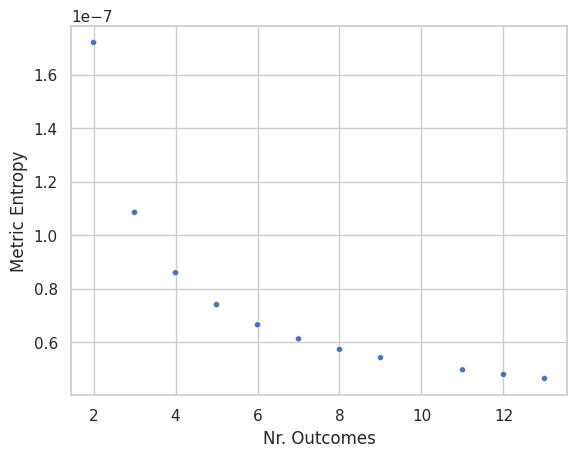
\includegraphics{figures/analysis/codex-s_scatter_nr_types_vs_metric_entropy.png}
        \caption{Type-attentive}
    \end{subfigure}
    \begin{subfigure}[b]{0.489\columnwidth}
        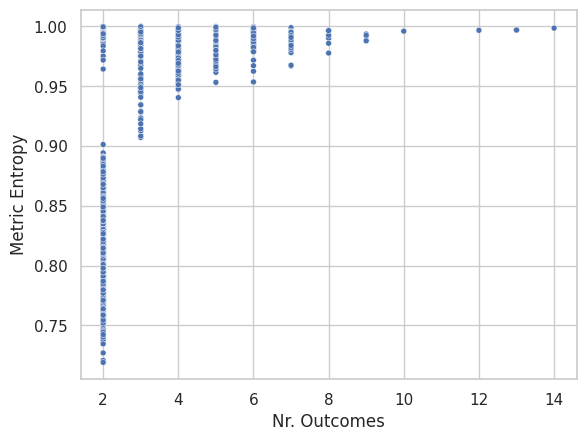
\includegraphics{figures/analysis/codex-s_alt_scatter_nr_types_vs_metric_entropy.png}
        \caption{Type-attentive-alt}
    \end{subfigure}
    \label{fig:metric_entropy_vs_nr_types_attentive_codex_s}
\end{figure*}

The intuition behind the type-attentive method was to have a weighted average between type representations rather than a simple mean. Like the type-mean method we see unexpectedly high MRR for the type-attentive method. We see even higher performance for this method, now for FB15K-237 too. In all likelihood because of similar reasons as the type-mean's high performance. This method can do even better at representing the type-statistics by learning to pick the one type that is most representative of each entity using the attention mechanism. To confirm this is the case we look at the attention weights as a probability distribution, and measure its Shannon Entropy to determine if most attention is paid to one or a few types or if the attention is fairly spread out.


%
In Figure \ref{fig:metric_entropy_vs_nr_types_attentive_codex_s} we can see a scatter plot of the Metric Entropy\sidenote[][2.2cm]{Metric Entropy is a normalized variant of the regular Shannon Entropy. It is obtained by dividing the Shannon Entropy by the information length (in bits, i.e. $log_2(|X|)$ where $|X|$ is the number of possible outcomes of the random variable). } of the attention weights for the type-attentive and type-attentive-alt methods when applied to the CoDEx-S dataset. We can see that the type-attentive method is assigning very low entropy weights to the type-vectors, regardless of the number of types of the entity\sidenote[][]{Note that for the type-attentive method the number of outcomes is often one (because that entity has only one type). These cases are not displayed in the plot, as Metric Entropy is undefined in those cases.}. This confirms that the the type-attentive method is choosing one type for each entity, using the type-statistics only to achieve high predictive performance.
%
The entropy for the type-attentive-alt variant looks rather different, its attention distributions are relatively high entropy.
This time the method seems to operate more like intended, taking in information from a variety of its types. Unfortunately, with an MRR that is slightly below the non-semantic baseline, this does not result in an increase in performance.

%
\begin{figure*}[t]
    \vspace{0.5cm}
    \centering
    \caption[Scatter plot of metric entropy for CoDEx-M.]{Scatter plot of metric entropy over the number of outcomes for the CoDEx-M dataset.}
    \begin{subfigure}[b]{0.50\columnwidth}
        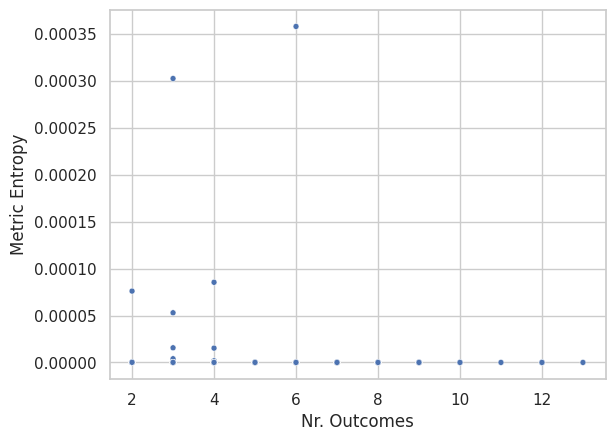
\includegraphics{figures/analysis/codex-m_scatter_nr_types_vs_metric_entropy.png}
        \caption{Type-attentive}
    \end{subfigure}
    \begin{subfigure}[b]{0.492\columnwidth}
        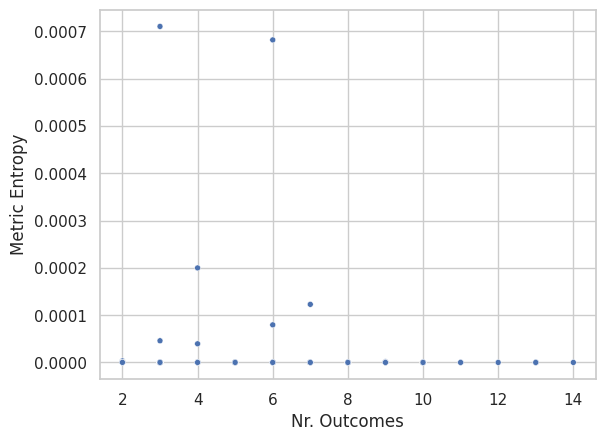
\includegraphics{figures/analysis/codex-m_alt_scatter_nr_types_vs_metric_entropy.png}
        \caption{Type-attentive-alt}
    \end{subfigure}\vspace{-1em}
    \label{fig:metric_entropy_vs_nr_types_attentive_codex_m}
\end{figure*}
%
In Figure \ref{fig:metric_entropy_vs_nr_types_attentive_codex_m} we can see the same type of plot but for the CoDEx-M dataset. Here we see that entropy is low for both of the method's variants, which explains why performance for both is similar. It seems that in rare cases even the type-attentive-alt method can uncover this type-statistics only mode where it attends only to a single representative type.


% \todo[inline,caption={}]{
%     \begin{itemize}
%         \item type attentive most attended as label for the types in TSNE
%     \end{itemize}
% }

\begin{table}%
    \def\fn{\hspace{2pt}} % footnote columns
    \setlength{\tabcolsep}{5pt}%
    \centering%
    \begin{tabular}{lr@{\fn}lr@{\fn}lr@{\fn}l}%
        \toprule%
                        &\multicolumn{2}{c}{FB15K-237}   %
                                           & \multicolumn{2}{c}{CoDEx-S}   %
                                                                & \multicolumn{2}{c}{CoDEx-M} \\
        \cmidrule{1-7}
        lr (default)    & $3.6 \cdot 10^{-2}$ && $1.7 \cdot 10^{-4}$ && $3.6 \cdot 10^{-2}$ \\
        lr (attn)       & $3.9 \cdot 10^{-1}$ && $6.6 \cdot 10^{-1}$ && $3.9 \cdot 10^{-1}$ \\
        \bottomrule
    \end{tabular} %\vspace{1em}
    \caption{Type-attentive learning rates for runs with best MRR.} %
    \label{tab:type-attn-lr}%
\end{table}%
%
\subsection{Type-attentive: hyper-parameters}\label{sec:analysis:type_attn_hparams}
In Table \ref{tab:type-attn-lr} we can see that the attention mechanism's learning rate is tuned to a higher value than we see for the rest of the model. 
The original intent of the separately tuned learning rate was to allow the attention mechanism to use a lower learning rate, not higher. It is possible that these learning rates play a role in reaching the low entropy modes.
%
The mutual information hyper-parameter was set below zero (disabled) for each dataset.

\subsection{Type-embedprior: learned distributions} \label{sec:analysis:type_embed_dist}
The intuition behind this method is that entities of the same type are similar, and should therefore be close to each other in the embedding space. Specifically, we construct distributions for each type and want the embedding of entities of those types to be likely under those distributions, and only those distributions.
To measure how well the learned distributions match this intuition, we now look at the degree of overlap between distributions. We hope that the distributions of types that do not have any entities in common also do not overlap in the embedding space.
We quantify the extent to which types have entities in common with the Jaccard Index, and  the degree of overlap with the Bhattacharyya Coefficient.

\begin{figure}
    \centering                             % left bottom right top
    \includegraphics[width=1.05\textwidth, trim=2mm 2mm 4mm 4mm, clip]
    {figures/analysis/embedprior/fb15k-237_scatter_typepair_jaccard_vs_bhattacharyya.png}
    \caption[Plot depicting Jaccard index of type pairs with the Bhattacharyya Distance between the learned distributions of those pairs.]{Combination of scatter plot, univariate KDE curves, and a linear regression fit, depicting the relation between the Jaccard Index of type pairs (as measured when considering types as sets of entities), and the Bhattacharyya Coefficient between the learned type distributions of said type pairs.}
    \label{fig:embedprior_jaccard_vs_bhattacharyya}
\end{figure}
A scatter plot of type-pairs with these two quantities on the x- and y-axis respectively can be seen in Figure \ref{fig:embedprior_jaccard_vs_bhattacharyya}. This figure also shows a linear regression fit, and displays the cardinality of the union of the two type sets using the color of the points, where bright yellow are the lowest and dark blue the highest cardinality\sidenote[][]{To reduce the total number of points and improve the utility of the plot, type-pairs with a Jaccard Index below 0.1 were left out. As were type-pairs with fewer than 10 entities between them, and types paired with themselves.}.
We see a clear correlation between the two quantities, but also see that it is mostly one-way. In an ideal scenario the points in the plot would form a diagonal line, showing perfect correlation. Instead, we observe that most points occur above this hypothetical line. This indicates that types with a lot of entities in common also overlap in the embedding space, but types that do not have many entities in common, may still overlap considerably in the embedding space. We also observe that the type-pairs with the most entities between them exhibit more overlap in the embedding space, which is to be expected.


\subsection{Type-embedprior: hyper-parameters}\label{sec:analysis:type_embed:hparam}
The type-embedprior embedder seeks to make the entity-embeddings likely under their type-distributions. To do this it uses a minimum constraint on log-density assigned by the correct types minus the log-density assigned by other types. In other words, an entity's true types must assign at least some number of times more density to the entity's embedding, than other types do.
\begin{table}
    \def\fn{\hspace{2pt}} % footnote columns
    \setlength{\tabcolsep}{5pt}
    \centering
    \begin{tabular}{lr@{\fn}lr@{\fn}lr@{\fn}lr@{\fn}l}
        \toprule
                &\multicolumn{2}{c}{WN18RR}
                            &\multicolumn{2}{c}{FB15K-237}   
                                           & \multicolumn{2}{c}{CoDEx-S}   
                                                                & \multicolumn{2}{c}{CoDEx-M} \\
        \cmidrule{1-9}
        min log-density $\Delta$ & 6.982 && 7.470 && 7.470 && 6.588 \\
        \bottomrule
    \end{tabular} %\vspace{1em}
    \caption[Differences in log-density required of entity-embedding under type distributions.]{Minimum difference in log-density required of entity-embedding under the distributions of that entities types and set of sampled negative types (for the best performing model from the hyper-parameter search).} \label{tab:min_log_density_delta}
\end{table}

In Table \ref{tab:min_log_density_delta} we can see the value of the hyper-parameter that governs the minimum difference in log-density required, for the best run from the hyper-parameter search.
We can see that for each dataset a similar value is selected. 
\begin{figure*}
    \centering
    \begin{subfigure}[b]{0.50\columnwidth}
        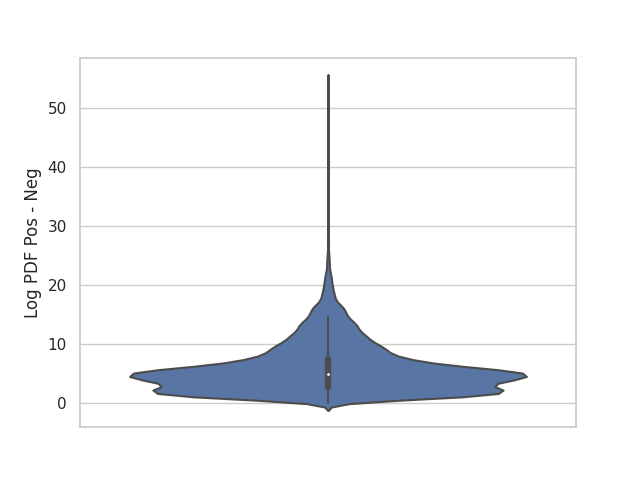
\includegraphics[trim=0cm 11mm 1cm 0pt, clip]{figures/analysis/embedprior/fb15k237_analysis_prior_lpdf_diff.png}
        \caption{FB15K-237}
    \end{subfigure}
    \begin{subfigure}[b]{0.492\columnwidth}
        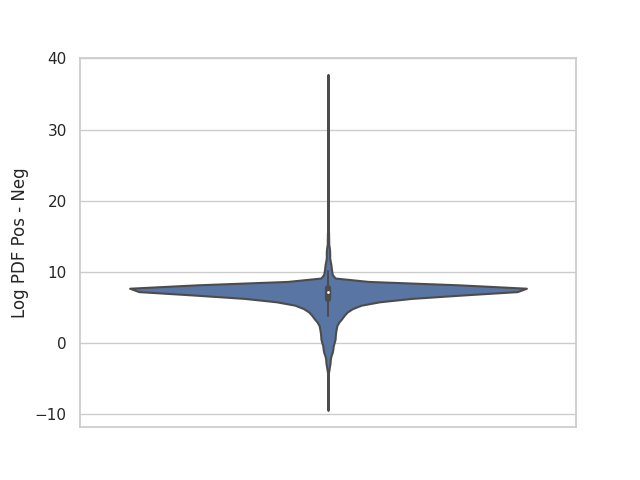
\includegraphics[trim=0cm 11mm 1cm 0pt, clip]{figures/analysis/embedprior/wnrr_analysis_prior_lpdf_diff.png}
        \caption{WN18RR}
    \end{subfigure}
    \begin{subfigure}[b]{0.492\columnwidth}
        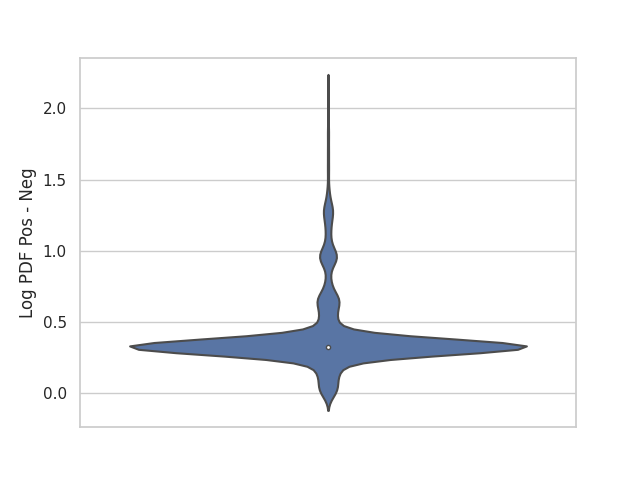
\includegraphics[trim=0cm 11mm 1cm 0pt, clip]{figures/analysis/embedprior/codex-s_analysis_prior_lpdf_diff.png}
        \caption{CoDEx-S}
    \end{subfigure}
    \begin{subfigure}[b]{0.492\columnwidth}
        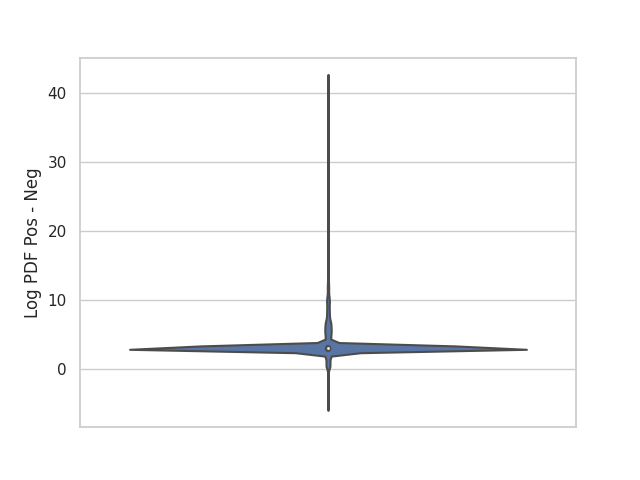
\includegraphics[trim=0cm 11mm 1cm 0pt, clip]{figures/analysis/embedprior/codex-m_analysis_prior_lpdf_diff.png}
        \caption{CoDEx-M}
    \end{subfigure}
    \vspace{-1em}
    \caption[Difference in density between positive and negative types.]{Difference in log-density between positive and negative types.}
    \label{fig:embedprior_lpdf_diffs}
\end{figure*}
However, as can be seen in Figure \ref{fig:embedprior_lpdf_diffs}, the actual difference in log-density that is obtained by the best performing checkpoint for each dataset does differ.
For FB15K-237 and WN18RR we can see that the constraint is satisfied for a lot of entities but not all. For the CoDEx datasets we can see that the constraint is violated for all entities.

